%!TEX root = ../main.tex

\section{Analysis} \label{sec:analysis}
In this chapter we will analyze further on the points brought up in the investigation. 
We will analyze Pac-Man in detail to find the parameters and inner mechanics of the game that we can manipulate using the genetic algorithm (GA).
Furthermore we will investigate how others have identified the performance of the players in order for the GA to know how the player is doing.
Finally we will analyze genetic algorithms further and define the areas that need to be implemented in order to get a functioning genetic algorithm. 


The following content about the original Pac-Man and it's implemented mechanics, pathfinding system and game parameters are presented to account for the original implementation of the game. Thus we can utilize the content to account for our interpretations and evaluations of player performance as specified in the final problem statement. This is a description of the original Pac-Man released in 1980's. \cite{Pittman2011}

% Pac-man content research


\subsection{Pac-man}\label{ssec:pacmandetail}
\subsubsection{Technical details/mechanics/paramters}

\textbf{About}\\
Pac-man is an arcade game which was developed by the company Namco, and was first released in 1980s.

Extensive documentation and descriptions of Pac-man have been accounted for by Pittmann, 2011.~\cite{Pittman2011}.

\textbf{Purpose}
The general purpose of the game is to control Pac-Man through a maze while gathering dots. Once all the dots within the maze have been collected by Pac-Man, the player proceeds to the next level. There are 255 levels in total.

While trying to proceed to the next level by collecting dots, there are also several other incorporated features.

\begin{figure}[!htbp]
\centering
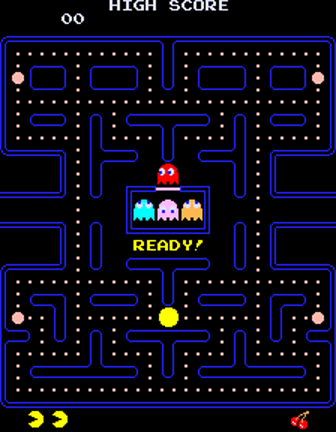
\includegraphics[scale=0.5]{pacman_level.png}
\caption{Pac-man level screenshot: \cite{Pittman2011} }
\label{fig:Pac-man}
\end{figure}


On figure \ref{fig:Pac-man}, the setup for a level is displayed. The following elements in the game, within a single level, are the following:

\begin{itemize}
\item Maze\\
The maze is the area of which the Pac-man and ghosts navigate around throughout a level. There exists many different mazes which depends on the version of Pac-Man.
\item Pac-Man\\
Pac-Man is the playing agent that is navigated throughout the levels by moving up, down, left and right.
\item Ghosts\\
The ghosts, as seen on figure \ref{fig:Pac-man}, is Blinky, Pinky, Inky and Clyde. They emerge from the center of the maze and chase the Pac-man throughout the level, each using unique behaviors to catch him. Description of the ghost behaviors can be found in section \ref{ssec:ai_behavior}.
\item Dots and energizers\\
The dots within the maze functions as the foundation for winning a level in Pac-man. Once all the dots are picked up/eaten by Pac-Man, the level is won.

The dots do however also grant points to the player.

Each dot is worth 10 points. In the original game, as stated by Pittman, 2011 \cite{Pittman2011}, there are 240 dots in total which amounts to 2400 points.

Energizers, which can be seen on figure \ref{fig:Pac-man} as 4 bigger dots placed in each corner of the maze also grant 50 points each.
In combination, the total amount of points acquired by dots and energizers are 2600. The energizers do however also alter the state of the ghosts into a mode of which it is possible for Pac-Man to eat the ghosts and thereby also acquire points for a limited amount of time.

While the ghosts remain in the state of "fleeing" caused by the Pac-man eating the energizer, each consecutive eaten ghost will result in twice as many points as the previous eaten ghost, whereof the first ghost gains the player 200 points.

If the player successfully eats all four ghosts wile the "fleeing" state is active, the player acquire a total of 3000 points.

If all ghosts are consumed under the "fleeing" state of each energizer, in combination with the points from the gathered dots the combined score is 14600.
\item Fruits\\
The fruits in Pac-Man are bonus elements that appear in the maze at certain times through a level which also adds points to the player, if collected. The fruit appears twice in each level and spawns when a certain amount of dots has been eaten.
The amount of points gained from the fruits range from anything from 100 to 5000 points, depending on the type of fruit that spawns. Also worth mentioning is that the fruit disappears after a certain amount of time if not consumed in time.
\end{itemize}

%!TEX root = ../../main.tex

\subsubsection{AI Pathfinding}\label{ssub:pathfinding}
The ghost AI of the original Pac-Man is based on a single pathfinding algorithm which all the modes previously discussed in the investigation utilizes \cite{Pittman2011}.
In order to get a better understanding of how these modes work we need to look at this pathfinding mechanism.

The maze is split up in tiles in a grid.
This grid has a size of 28 x 36 tiles, this includes everything on the screen including score counters, and life count.
The size of the individual tiles depends on the resolution of the game space.
In the case of the origin Pac-Man the screen size was 224 x 288 pixels.
That makes each tile 8 x 8 pixels in size.

The pathfinding works by finding a path from one tile to the other using only the tiles that are walkable within the maze.
Tiles outside the maze and tiles with pieces of wall within them, while still tiles in the collection of tiles, are considered illegal tiles.

\begin{figure}[!htbp]
\centering
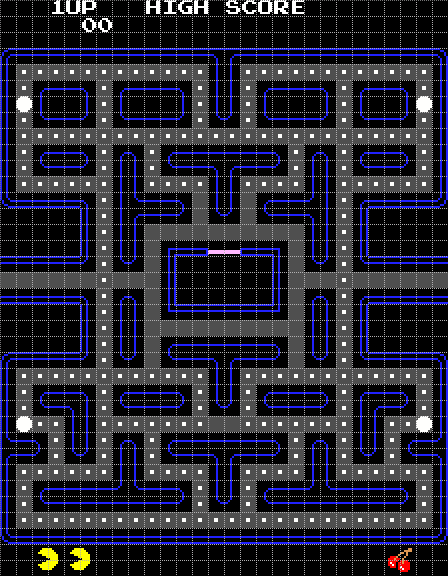
\includegraphics[width=0.5\textwidth]{Tiles.png}
\caption{Visible space in a game of Pac-Man: \cite{Pittman2011} }
\label{fig:Pacman_visible_space}
\end{figure}

While the ghost can only move along a path using legal tiles, the ghosts target tile can be anywhere on the grid.
In chase mode the target tile will be somewhere near the Pac-Man (depending on the ghost in question), and in scatter mode where the ghost will move towards its designated corner of the maze.
The target tile the ghost will go to when in scatter mode is fixed outside of the maze to ensure that the ghost will never get to it, resulting in the ghost circulating in the area closest to the fixed target until it has a new target.
Another fixed tile is the one in the ghost-one in the middle of the screen.
This is activated when the ghost has been eaten by the Pac-Man and is sent back to the pen.

In Figure \ref{fig:Pacman_visible_space} we can see the grid laid out over the screen of Pac-Man. The grey tiles are considered legal and the tiles that the pathfinding works with. The eatable pellets are the white dots in the middle of those tiles.

The bulk of the pathfinding happens when the ghost reaches an intersection in the maze.
When the ghost is one tile away from an intersection, it will adjust its direction.
It works by finding the tile with the shortest distance to the target.
It looks one ahead in every direction of the intersection and chooses whichever direction has the shortest distance to the target.
When a ghost is presented with a tie, meaning an intersection where two or more directions have equal distance to the target, the ghost will default to choosing the direction in a specific order: \emph{up, left, down, right}\cite{Pittman2011}.
This means that when the ghost is in a tie situation it will always choose the an upwards direction before left, if those two were the tie directions.


\subsubsection{AI behavior}\label{ssec:ai_behavior}
Even though the ghosts all share the same modes, the implementation of specifically chase mode is different for each ghost.

\subsubsection*{The red ghost (Blinky)}
The red ghost is the most aggressive of the four, and is described as \emph{the shadow}. His chase mode uses Pac-Man's current tile as the target tile, which makes him difficult to shake off when he is close. Also implemented is “Cruise Elroy” mode. Twice each round, Blinky will turn into Elroy. This is determined by the number of pellets left in the maze. When Blinky turns into Elroy, he will become faster; first time as fast as the Pac-Man, and the second time he will be faster. His scatter mode is also changed when in Elroy mode, instead of wandering the maze aimlessly, he will continue to chase the Pac-Man. He will turn around and leave the Pac-Man until an intersection is reached.

\subsubsection*{The pink ghost (Pinky)}
When in chase mode, Pinky will not use the Pac-Mans current tile as the target, instead his target is four tiles in front of the Pac-Man. His mission is therefore to cut the Pac-Man off and box him in. Interestingly when the Pac-Man is walking to the top of the maze, Pinkys target changes from four tiles ahead to four ahead \textit{and} four to the left. This is because of a bug in the code that was not fixed.

\subsubsection*{The blue ghost (Inky)}
Inky can be seen as one of the more dangerous of the four. Instead of having just one targeting scheme, he seems to switch between the schemes of his comrades, sometimes chasing, sometimes blocking off or even wandering effortlessly. As with Pinky, Inky also uses an offset tile two tiles in front of Pac-Man. Inky also uses Blinkys position in regard to the Pac-Man to determine his target tile. This has the effect that Inky will be close to the Pac-Man whenever Blinky is close to the Pac-Man and vice-versa.

\subsubsection*{The orange ghost (Clyde)}
Clyde seems to stay away from the Pac-Man and do his own thing. He uses the distance to the Pac-Man to determine his target tile. If he is far from the Pac-Man he will go into chase mode just as Blinky would. When he comes within eight tiles of the Pac-Man he will turn around and go into scatter mode. While Clyde will never reach the Pac-Man on his own, he can still be dangerous if the Pac-Man gets in his way for instance during scatter mode.


\subsection{Player performance(PP)}\label{ssec:player-performance}

As described in the final problem statement, we try to implement a genetic algorithm that corresponds to the player's performance in Pac-Man.


The aim of identifying player performance, is to focus on the specific game parameters, mechanics and functionalities within Pac-Man to access the performance of the player. We observe elements within the game, which might give some indication as to how the player is performing.

In section \ref{ssec:ga}, we account for the usage of genetic algorithms. It is in section \ref{ssec:ga} how the evaluation of a fitness function is conducted. How it is defined largely depends on the problem at hand. There are no single solution to how a given problem can be evaluated by a fitness function, and these properties are transferable to the purpose and ability to identify player performance in Pac-Man.

There are however several examples of how some implementations of genetic algorithms in Pac-Man are accessed to account for their implemented fitness function. Such implementations can provide knowledge of how one might try to evaluate upon player performance.

In the research of Lucas, 2005 \cite{Lucas2005}, he mentions how further directions of research might point towards assignment of fitness scores based upon the objective of ghosts, whereof the fitness is assigned to ghosts that tries to minimize the possible attainable score of Pac-Man.

In the research conducted by Simon and Kalyanpur, 2001 \cite{Kalyanpur2001} they simply assigned the highest fitness score to the ghost that actually caught Pac-Man.

Additionally in the research of Gallagher and Ledwich, 2007 \cite{Gallagher2007}, they calculate the fitness based upon some average amount of points in a game of Pac-Man in some averaged percentage over several generations.

As there are no conclusive outcome as to how one might access player performance, there are several criteria which can be outlined that will make a selection of possible player performance criteria possible.

\begin{itemize}
\item Game parameters.\\
Such as points acquisition and successful completion of objectives or failures of not completing said objectives.
\item Method of conduction.\\
How the actual completions or failures are conducted. Time spent up until completion or failure and the general method of attaining such results. Examples are, what directions were utilized, when did specific actions or choices occur. A general appraisal of the method to reach any specified goal.
\end{itemize}

Therefore, a specification of player performance will be decided, in the design chapter, see section XX, based upon the chosen implementation of genetic algorithms in Pac-man.




\subsection{Genetic Algorithm(s)}\label{ssec:ga}

\subsubsection{Description}
Genetic algorithms were invented by John Holland in 1975 and is proposed as a heuristic method, which is a method to learn by itself based upon survival of the fittest, where it is described as a  search algorithm that uses mechanisms much like evolution to improve some solutions to a given problem. \cite[pp. 20]{Sivanandam2008}

The Genetic Algorithm starts with a set of plausible solutions and by the use of genetic operator alterations like reproduction, crossovers and mutations \cite{Baltzer2014}, it develops a new set of better solutions compared to the previous. By repeating this process, a population will theoretically improve until a satisfying result is found to the given problem. \cite{BCS2013}

It is noteworthy about "satisfying results" is that we search for some better solution within a set of possible solutions, also referred to as search space. It is therefore not guaranteed to find some, if any, optimal solution to the problem but rather a/some solution(s) which can be interpreted as acceptable. \cite[pp. 20/21]{Sivanandam2008}


In genetic algorithms, populations and individuals covers the terminology of the solutions and searches thereof. An individual is to be considered a single solution to the problem and the population is the number of individuals involved. \cite[pp. 39]{Sivanandam2008}



\subsubsection{Genetic Algorithm Components}

A Genetic Algorithm consists of at least five components as described by Baltzer, 2014 \cite{Baltzer2014}. These components can be considered to be the main components in any genetic algorithm.


\subsubsection*{Chromosome / gene representation}

A representation of a population and the subordinate content, being chromosomes and genes as seen on figure \ref{fig:gene}.
The genes function as a string of some arbitrary length of data. A chromosome is a sequence of genes, where the combined chromosomes serve as the population. \cite[pp. 41]{Sivanandam2008}

As mentioned above, each individual(chromosome) is a single solution to the problem at hand. The chromosomes can be considered to be \enquote{a point in the search space of candidate solutions} \cite[pp. 7]{Melanie1990} Melanie, 1990.


\begin{figure}[!htbp]
\centering
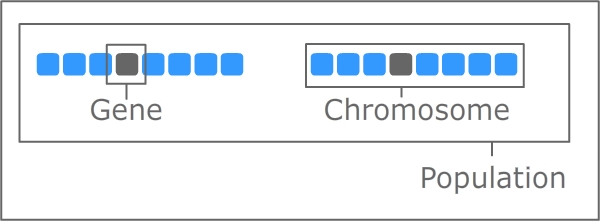
\includegraphics[scale=1.0]{gene_chromosomes.jpg}
\caption{gene, chromosomes and population description}
\label{fig:gene}
\end{figure}

The chromosomes which contains an array of genes is an abstract representation of data. Thus the chromosomes and genes must be encoded in some way, dependent on the problem. It is basically a method of representing the individual genes, which translates into the data.
There are several ways that the genes can be encoded. Some of the encoding methods are listed by Obitko, 1998 \cite{Marek1998} and by Sivanandam, 2008 \cite[pp.43]{Sivanandam2008}

The types of encoding methods are as follows:
\begin{itemize}
\item Binary encoding
\item Octal encoding
\item Vexadecimal encoding
\item Permutation encoding(sequence of numbers)
\item Value encoding(string of values. numbers, letters, strings etc)
\item Tree encoding(every chromosome is a tree of some objects)
\end{itemize}


\subsubsection*{Initialization of the population}

A population is a collection of individuals(chromosomes).

An initial population must be created as a starting point for the algorithm. This representation of a population is chosen randomly, as there might be no prior evident solutions. Dependent on the stated problem at hand, the initialization of populations might also be carried out with some good solutions to the problem. However in most cases, the initial population is chosen at random. \cite[pp. 41/42]{Sivanandam2008}


\subsubsection*{Evaluation function(fitness)}

In order to improve further generations, the fitness of each chromosome in the current population must be evaluated. The genetic algorithm does so by the use of a fitness function, which assigns some score(fitness) to each of the chromosomes within a specific population.
In general manners, the fitness of a given chromosome is dependent on how succesfully the given chromosome solved the designated problem, and is conveyed through a range of values. The better the solution, the higher the fitness score. \cite[pp. 8]{Melanie1990}

How "good" the solution is, is the whole purpose of the fitness function to identify. The fitness function performs some evaluation of the acquired results and then assigns a specific fitness score to that solution. How the fitness function performs the evaluation of a solution is dependent on the problem itself. There are no single solutions as to how the fitness function is to be developed, but can really be anything, that succesfully covers the plausible methods of evaluating the solutions. \cite[pp. 31]{Sivanandam2008}

\subsubsection*{Genetic operators altering chromosomes(reproduction/selection, crossover and mutation.}


Genetic operators in some of the more simple Genetic Algorithms are reproduction/selection, crossover and mutation. Melanie, 1990. \cite{Melanie1990}

\textbf{Reproduction/selection:} \enquote{This operator selects chromosomes in the population for reproduction. The fitter the chromosome, the more times it is likely to be selected to reproduce.} \cite[pp. 8]{Melanie1990}
The idea behind this operator is that preferences are given to the better chromosomes in the population, which is then passed on to the next generation. This is based upon the fitness score.

Within the selection operator, several selection methods exists which defines how the actual selection of "best" individuals is to be conducted.

Some of the selection methods are:
\begin{itemize}
\item Roulette Wheel Selection
\item Random Selection
\item Rank Selection
\item Tournament Selection
\item Boltzmann Selection
\item Stochastic Universal Sampling
\item Steady-State Selection
\item Elitism
\item Fitness Proportionate selection
\item Scaling Selection
\item Generation Selection
\item Hierarchical Selection
\end{itemize}
The list is from Sivanandam, 2008 \cite[pp. 46-50]{Sivanandam2008} and Markzyk, 2004 \cite{Adam2004}.

The different selection methods will not be accounted for and described in this chapter, however the appropriate selection method will be addressed in the design chapter along with descriptive reasoning and method of application of the selected method(s), or combination of such.


The crossover method takes two parent solutions(chromosomes) to create new individuals, by swapping genes between two of the potentially good solutions. There exists several crossover methods, which are:


\begin{itemize}
\item Single Point Crossover
\item Two Point Crossover
\item Multi-Point Crossover (N-Point crossover)
\item Uniform Crossover
\item Three Parent Crossover
\item Crossover with Reduced Surrogate
\item Shuffle Crossover
\item Precedence Preservative Crossover (PPX)
\item Ordered Crossover
\item Partially Matched Crossover (PMX)
\end{itemize}
The list is from Sivanandam, 2008 \cite[pp. 50-56]{Sivanandam2008}

Similarly with the list of selection operators, we will not account for the crossover operator methods, but will be addressed in the design chapter with similar procedures and content.

Additionally with the crossover operator, we can describe the crossover probability.
The crossover probability is a parameter that describes the likelihood of crossover. It basically states how often that the crossover method will be performed.\cite[pp. 56]{Sivanandam2008}

The crossover probability determines how the new generation (offspring) is altered. If there is some crossover probability then the offspring will contain genes from both of the parent chromosomes. If there is no crossover probability then the offspring will be copies of the parent chromosomes. They will be exact copies, but does not mean that they are the same.


\textbf{Mutation:} \enquote{This operator randomly flips some of the bits in a chromosome.} \cite[pp. 8]{Melanie1990}

The mutation operator happens after the crossover operator. The mutation randomly alters the structure(ordering of the genes) within the chromosomes or randomly modifies it.
The mutation of the chromosomes can happen in the following manners, dependent on the kind of representation of genes; flipping, interchanging and reversing.\cite[pp. 57]{Sivanandam2008}

Flipping genes/values is simply alterations of some to other, and other to some which then indicates a child from that chromosome. Example can be that a gene(1) is converted to gene(0), and gene(0) is converted to gene(1).

Interchanging is randomly assigning two genes within a chromosome and then switch locations of the two genes.

Lastly, reversing is randomly choosing a gene within a chromosome and thereafter change the location of the gene with a gene next to it.

Much like crossover probability, there is also a mutation probability. It states how often parts of the chromosome will be mutated. If a mutation occurs, then the chromosome is changed, in some way as specified above. If the mutation probability is 0 percent, then no mutation occurs and if the mutation is at 100 percent, then the whole chromosome is changed in accordance with the type of mutation that is specified. The reason to implement mutation of the chromosomes is to ensure that the genetic algorithm does not fall into some local extremes.\cite[pp. 57]{Sivanandam2008}

\subsubsection{Parameters for population size and probabilities of genetic operators.}


The population size covers the amount of solutions(chromosomes) that is in the actual population in the search space. The actual size of the population does very much depend on the problem at hand.\cite[pp. 42]{Sivanandam2008}


Another important aspect is the actual probability of the mutation and crossover operations.
It is mentioned in the appropriate sections concerning mutation and crossover what happens in in the absence(0 percent) or fully enabled(100 percent), but does not account for the most efficient percentage of the two. It is however also dependent on the problem, so finding some specific value, or range of values to a percentage of the crossover or mutation probability will not be possible to define, before the actual problem is defined along with some indications of plausible solutions.

The alterations in the probability may or may not have positive effects on the new generations of populations.

Marek, 1998\cite{Marek1998}  describes some recommendations based upon empirical studies which plausible can be used as a reference point, but can be considered to be general and not necessarily the most optimal configurations, so alterations and adjustments must be conducted to account for the specific problem at hand.

The general recommendations are described as followed:
\begin{itemize}
\item Crossover rate: 80-95 percent.

It is however mentioned that occurrences of crossover probabilities of 60 percent was optimal in some undefined problem scenarios.
\item Mutation rate: 0.5-1.0 percent

The mutation rate is described as being optimal when very low.
\item population size

It is described that population size very much depend on encoding and size of the chromosomes. A population size of 20-30 is stated as good, but other examples of 50-100 are also accounted for as a good population size.
\end{itemize}

\subsubsection{Genetic algorithm procedure}


Now that the general usage, definition and components has been described, a short general description of the procedure as to implementation and functionality of a general algorithm can be defined.

Each iteration of the genetic algorithm process is defined as a generation. The entire set of generations is defined as a run. \cite[pp. 9]{Melanie1990}





A general genetic algorithm is here defined algorithmically by Malhotra et.al, 2011 \cite[pp. 40]{Rahul2011}, much similar is that of Sivanandam, 2008 \cite[pp. 30-31]{Sivanandam2008}
\enquote{
\begin{description}
\item[Start:] Generate population of chromosomes.
\item[Fitness:] Evaluate fitness score of each chromosome in the population.
\item[New Population:] Create new population of solutions by repeating the following steps until the new population is created.
\begin{description}
\item[a:] Select parent chromosomes based upon the fitness score.
\item[b:] Use the crossover operator on the parents to form new children.
\item[c:] Use the mutation operator to mutate the children.
\item[d:] Place the children into the new population.
\end{description}
\item[Replacement:] Use the new generation in the algorithm.
\item[Test:] If the success criteria/conditions is met, terminate the algorithm and return the solution in the population.
\item[Loop:] Return and run step 2.
\end{description}
} \cite[pp. 40]{Rahul2011}



\subsubsection{Summary}
In section \ref{ssec:pacmandetail}, we describe the mechanics and implemented features of Pacman in order to account for a plausible implementation to use as a test bed for the attended in-cooperated genetic algorithm. To do so, we have researched the theories and methods of actual applications of genetic algorithms. The combination of acquired research  will allow us to combine the content of Pacman with the necessities of an implemented genetic algorithm in order to successfully answer to the final problem statement.

Furthermore we account for the formulation of fixed behaviors in section \ref{ssec:ai_behavior}.

Lastly, we find that interpretation of player performance is problem dependent, and the actual assessment will be accounted for in the design chapter, see chapter \ref{ssec:player-performance}.